%%%%%%%%%%%%%%%%%%%%%%%%%%%%%%%%%%%%%%%%%
% Academic Title Page
% LaTeX Template
% Version 2.0 (17/7/17)
%
% This template was downloaded from:
% http://www.LaTeXTemplates.com
%
% Original author:
% WikiBooks (LaTeX - Title Creation) with modifications by:
% Vel (vel@latextemplates.com)
%
% License:
% CC BY-NC-SA 3.0 (http://creativecommons.org/licenses/by-nc-sa/3.0/)
%
%%%%%%%%%%%%%%%%%%%%%%%%%%%%%%%%%%%%%%%%%

%----------------------------------------------------------------------------------------
%	PACKAGES AND OTHER DOCUMENT CONFIGURATIONS
%----------------------------------------------------------------------------------------

\documentclass[11pt]{article}

\usepackage[utf8]{inputenc} % Required for inputting international characters
\usepackage[T1]{fontenc} % Output font encoding for international characters
\usepackage{mathpazo} % Palatino font
\usepackage{amsmath}
\usepackage{tikz}
\usepackage{mathdots}
\usepackage{yhmath}
\usepackage{cancel}
\usepackage{color}
\usepackage{siunitx}
\usepackage{array}
\usepackage{multirow}
\usepackage{amssymb}
\usepackage{gensymb}
\usepackage{tabularx}
\usepackage{booktabs}
\usepackage[ruled,vlined]{algorithm2e}
\usetikzlibrary{fadings}
\usetikzlibrary{patterns}
\usetikzlibrary{shadows.blur}

\begin{document}

%----------------------------------------------------------------------------------------
%	TITLE PAGE
%----------------------------------------------------------------------------------------

\begin{titlepage} % Suppresses displaying the page number on the title page and the subsequent page counts as page 1
	\newcommand{\HRule}{\rule{\linewidth}{0.5mm}} % Defines a new command for horizontal lines, change thickness here
	
	\center % Centre everything on the page
	
	%------------------------------------------------
	%	Headings
	%------------------------------------------------
	
	\textsc{\LARGE Polytech Nice Sophia}\\[1.5cm] % Main heading such as the name of your university/college
	
	\textsc{\Large Projet SI4 - Algorithmes et Complexité.}\\[0.5cm] % Major heading such as course name
	
	\textsc{\large Rapport de projet}\\[0.5cm] % Minor heading such as course title
	
	%------------------------------------------------
	%	Title
	%------------------------------------------------
	
	\HRule\\[0.4cm]
	
	{\huge\bfseries Algorithmes pour l'inférence de connectivité avec application en biologie structurale computationnelle}\\[0.4cm] % Title of your document
	
	\HRule\\[0.6cm]

		
	%------------------------------------------------
	%	Logo
	%------------------------------------------------
	
	\vfill
	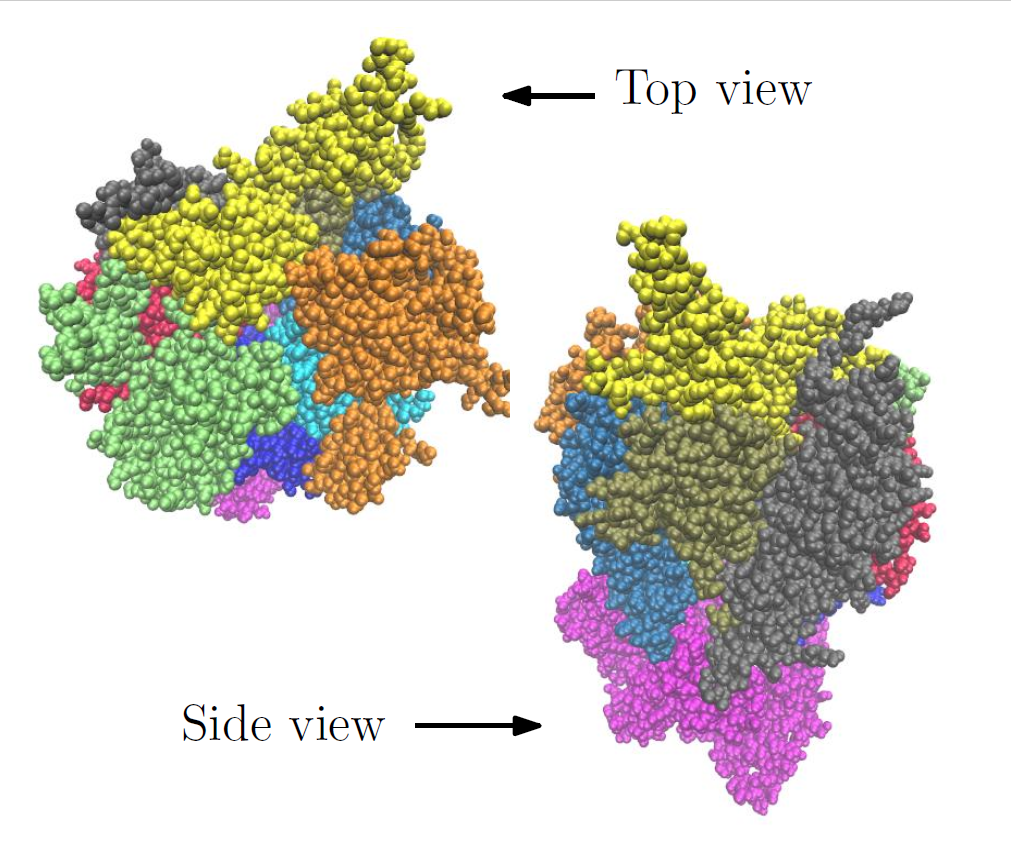
\includegraphics[width=0.6\textwidth]{complex.png}\\[1cm] % Include a department/university logo - this will require the graphicx package
	
	%------------------------------------------------
	%	Author(s)
	%------------------------------------------------
	
	\begin{minipage}{0.4\textwidth}
		\begin{flushleft}
			\large
			\textit{Author}\\
			Louis \textsc{Amas} % Your name 

			Maxime \textsc{Leras} % Your name
		\end{flushleft}
	\end{minipage}
	~
	\begin{minipage}{0.4\textwidth}
		\begin{flushright}
			\large
			\textit{Author}\\
			Pierre-Antoine \textsc{Boulat} % Supervisor's name
			Julien \textsc{Molinier} % Supervisor's name
		\end{flushright}
	\end{minipage}
	
	
	% If you don't want a supervisor, uncomment the two lines below and comment the code above
	%{\large\textit{Author}}\\
	%John \textsc{Smith} % Your name
	
	%------------------------------------------------
	%	Date
	%------------------------------------------------
	
	\vfill\vfill\vfill\vfill % Position the date 3/4 down the remaining page
	
	{\large\today} % Date, change the \today to a set date if you want to be precise

	 
	%----------------------------------------------------------------------------------------
	
	\vfill % Push the date up 1/4 of the remaining page
	
\end{titlepage}

%----------------------------------------------------------------------------------------

\newpage

\section{Question 1}
\paragraph{}
\begin{equation}
	Pour \; \Delta = 3 : 
\end{equation}

Une solution existe avec :

\begin{equation}
	\Delta(G) = deg({\widehat{S}_2}) = deg({\widehat{S}_4}) = 3
\end{equation}

\paragraph{}
\tikzset{every picture/.style={line width=0.75pt}} %set default line width to 0.75pt        

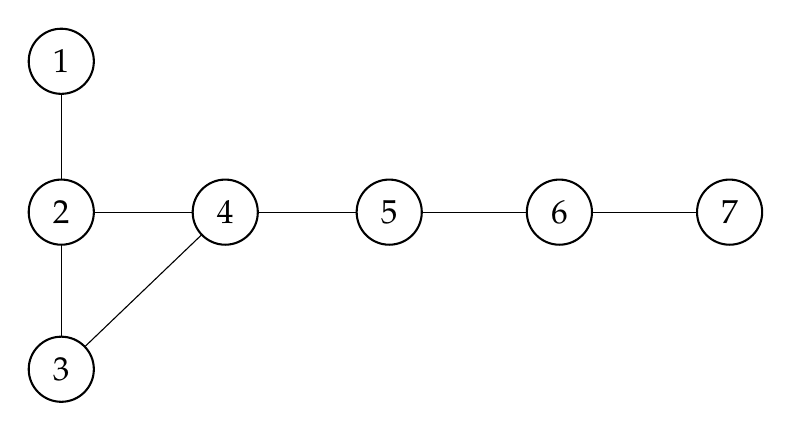
\begin{tikzpicture}[x=0.75pt,y=0.75pt,yscale=-1,xscale=1]
%uncomment if require: \path (0,232.6750030517578); %set diagram left start at 0, and has height of 232.6750030517578

% Text Node
\draw  [line width=0.75]   (168, 41.31) circle [x radius= 15.69, y radius= 15.69]   ;
\draw (168,41.31) node  [font=\large] [align=left] {1};
% Text Node
\draw  [line width=0.75]   (168, 189.69) circle [x radius= 15.69, y radius= 15.69]   ;
\draw (168,189.69) node  [font=\large] [align=left] {3};
% Text Node
\draw  [line width=0.75]   (168, 114) circle [x radius= 15.69, y radius= 15.69]   ;
\draw (168,114) node  [font=\large] [align=left] {2};
% Text Node
\draw  [line width=0.75]   (247, 114) circle [x radius= 15.69, y radius= 15.69]   ;
\draw (247,114) node  [font=\large] [align=left] {4};
% Text Node
\draw  [line width=0.75]   (326, 114) circle [x radius= 15.69, y radius= 15.69]   ;
\draw (326,114) node  [font=\large] [align=left] {5};
% Text Node
\draw  [line width=0.75]   (408, 114) circle [x radius= 15.69, y radius= 15.69]   ;
\draw (408,114) node  [font=\large] [align=left] {6};
% Text Node
\draw  [line width=0.75]   (490, 114) circle [x radius= 15.69, y radius= 15.69]   ;
\draw (490,114) node  [font=\large] [align=left] {7};

% Connection
\draw    (168,57) -- (168,98.31) ;
% Connection
\draw    (168,129.69) -- (168,174) ;
% Connection
\draw    (183.69,114) -- (231.31,114) ;
% Connection
\draw    (262.69,114) -- (310.31,114) ;
% Connection
\draw    (341.69,114) -- (392.31,114) ;
% Connection
\draw    (423.69,114) -- (474.31,114) ;
% Connection
\draw    (179.33,178.84) -- (235.67,124.86) ;

\end{tikzpicture}


\paragraph{}
\begin{equation}
	Pour \; \Delta = 2 : 
\end{equation}

	Pas de solution car les sommets 4 et 5 sont présent dans 3 sous complexes, 
	ce qui force un degrée minimal sur ces sommets de 3

\begin{equation}
	\left | C_b \cap C_c \cap C_d \right | = 2 \;\; < 3
\end{equation}

\section{Question 2}
\paragraph{}
Lorsque $\Delta = | V |$, il existe une solution au problème IC lorsque

\begin{equation}
	k \geq (\sum_{i=1}^{t} | C_i |) - t
\end{equation}

Ces valeurs de $k$ ne sont vraies qu'en faisant la supposition que 

$|C_i \cap C_j| \leq 1$ pour tout $i \in \left\{1,...,t\right\}$ et pour tout
 $j \in \left\{1,...,t\right\} , i\ne j.$

 \paragraph{}
 En effet, si on avait $|C_i \cap C_j| > 1$, la valeur de $k$ minimale pour que 
le problème IC ait une solution serait inférieure à la valeur donnée en (5)
	

\newpage
\paragraph{}
Si $k = |V|^2$, on observe qu'un graphe complet a au plus $\frac{n*(n+1)}{2}$ arrêtes où $n = |V|$

Or $\forall n \geq 1, \frac{n*(n+1)}{2} \leq n^2$ , Cela revient donc à ne pas se préoccuper de $k$ 
car $|E|$ ne pourra jamais être supérieur à $k$

Les valeurs de $\Delta$ pour lesquelles IC a une solution sont donc toutes les valeurs
supérieures ou égales au nombre maximal d'occurences d'un sommet dans tous les sous-complexes

\paragraph{}
Si on prend l'exemple d'un assemblage dont tous les sous-complexes contiennent le même sommet $\widehat{S}_1$,
toujours en respectant la supposition de l'énoncé : $|C_i \cap C_j| \leq 1$ pour tout $i \in \left\{1,...,t\right\}$ et pour tout
$j \in \left\{1,...,t\right\} , i\ne j.$

On obtient un graphe en forme "d'étoile" avec pour centre le sommet $\widehat{S}_1$. Pour que IC ait une solution
dans cette instance, il faut $\Delta = t$ car $t$ est le nombre maximal d'occurences d'un sommet dans les sous-ensembles
et ce sommet est ici $\widehat{S}_1$

\section{Question 3}
\paragraph{}
Le nombre d'abres couvrants différents pour un graphe complet $G(V,E)$ à $p$ sommets peut directement être calculé
avec la formule de Cayley et on obtient :

\begin{equation}
	a(G) = p^{p-2} 
\end{equation}

\paragraph{}
Le nombre de solutions différentes en fonction de la taille des $C_i$ si $\Delta = |V|$
est le produit des $p^{p-2}$ appliqués à chacun des sous-complexes (avec $p$ le 
nombre de sommets du sous-complexe).

\section{Question 4}
\paragraph{}
Les conditions d'existence d'une solution en supposant $\Delta=2$, $|C_i \cap C_j| \leq 1$ pour tout $i \in \left\{1,...,t\right\}$ et pour tout
$j \in \left\{1,...,t\right\} , i\ne j$ sont les suivantes :
\begin{itemize}
    \item Chaque protéine doit appartenir au maximum à 2 sous-complexes ayant
2 protéines au minimum
    \item Dans un sous-complexe, on ne peut pas avoir plus de 2 protéines si elles
appartiennent aussi à un autre sous-complexe.
\end{itemize}

\section{Question 8}
\begin{tabular}{ | l | l | l | l | l | l | l | l | l | l | l |}
	\hline
	$\Delta$ $k$ & 110 & 120 & 130 & 140 & 150 & 160 & 170 & 180 & 190 & 200 \\ \hline
	2 & 0 & 0 & 0 & 0 & 0 & 0 & 0 & 0 & 0 & 0 \\ \hline
	3 & 0 & 0 & 0 & 0 & 0 & 0 & 0 & 0 & 0 & 0 \\ \hline
	4 & 0 & 0 & 0 & 0 & 0 & 0 & 0 & 0 & 0 & 0 \\ \hline
	5 & 0 & 0 & 0 & 0 & 0 & 0 & 0 & 0 & 0 & 0 \\ \hline
	6 & 0 & 0 & 0 & 0 & 0 & 0 & 0 & $30\%$ & $10\%$ & $10\%$  \\ \hline
	7 & 0 & 0 & 0 & 0 & 0 & 0 & 0 & $20\%$  & $10\%$  & $10\%$  \\ \hline
	8 & 0 & 0 & 0 & 0 & 0 & 0 & 0 & $40\%$  & $90\%$  & $80\%$  \\ \hline
	9 & 0 & 0 & 0 & 0 & 0 & 0 & 0 & $70\%$  & $80\%$  & $90\%$  \\ \hline
	
	\hline
\end{tabular}

\section{Question 9}
\paragraph{}
Comme la limite de 200 arrêtes ne suffit pas et que certains tableaux ne contiennent que des 0 la limite a
été repoussé à 400 pour cette question.
\paragraph{}
$t =  20, p =  10$
\begin{center} \tiny \begin{tabular}{|l |l |l |l |l |l |l |l |l |l |l |l |l |l |l |l |l |l |l |l |l |} \hline
$\Delta$ $k$ &250 & 260 & 270 & 280 & 290 & 300 & 310 & 320 & 330 & 340 & 350 & 360 & 370 & 380 & 390 & 400 & 410 & 420 & 430 & 440  \\ \hline
1 & 0 & 0 & 0 & 0 & 0 & 0 & 0 & 0 & 0 & 0 & 0 & 0 & 0 & 0 & 0 & 0 & 0 & 0 & 0 & 0  \\ \hline
2 & 0 & 0 & 0 & 0 & 0 & 0 & 0 & 0 & 0 & 0 & 0 & 0 & 0 & 0 & 0 & 0 & 0 & 0 & 0 & 0  \\ \hline
3 & 0 & 0 & 0 & 0 & 0 & 0 & 0 & 0 & 0 & 0 & 0 & 0 & 0 & 0 & 0 & 0 & 0 & 0 & 0 & 0  \\ \hline
4 & 0 & 0 & 0 & 0 & 0 & 0 & 0 & 0 & 0 & 0 & 0 & 0 & 0 & 0 & 0 & 0 & 0 & 0 & 0 & 0  \\ \hline
5 & 0 & 0 & 0 & 0 & 0 & 0 & 0 & 0 & 0 & 0 & 0 & 0 & 0 & 0 & 0 & 0 & 0 & 0 & 0 & 0  \\ \hline
6 & 0 & 0 & 10\% & 0 & 0 & 0 & 0 & 10\% & 0 & 0 & 10\% & 0 & 10\% & 20\% & 10\% & 0 & 0 & 0 & 0 & 0  \\ \hline
7 & 20\% & 10\% & 20\% & 50\% & 10\% & 50\% & 20\% & 10\% & 30\% & 30\% & 20\% & 0 & 10\% & 10\% & 20\% & 0 & 0 & 0 & 0 & 0  \\ \hline
8 & 70\% & 50\% & 50\% & 70\% & 80\% & 70\% & 80\% & 100\% & 90\% & 70\% & 70\% & 70\% & 80\% & 50\% & 80\% & 0 & 0 & 0 & 0 & 0  \\ \hline
9 & 80\% & 70\% & 60\% & 80\% & 90\% & 90\% & 80\% & 80\% & 70\% & 90\% & 70\% & 90\% & 100\% & 80\% & 80\% & 0 & 0 & 0 & 0 & 0  \\ \hline
\end{tabular}\end{center}

\paragraph{}
$t =  20, p =  15$
\begin{center} \tiny \begin{tabular}{|l |l |l |l |l |l |l |l |l |l |l |l |l |l |l |l |l |l |l |l |l |} \hline
$\Delta$ $k$ &250 & 260 & 270 & 280 & 290 & 300 & 310 & 320 & 330 & 340 & 350 & 360 & 370 & 380 & 390 & 400 & 410 & 420 & 430 & 440  \\ \hline
1 & 0 & 0 & 0 & 0 & 0 & 0 & 0 & 0 & 0 & 0 & 0 & 0 & 0 & 0 & 0 & 0 & 0 & 0 & 0 & 0  \\ \hline
2 & 0 & 0 & 0 & 0 & 0 & 0 & 0 & 0 & 0 & 0 & 0 & 0 & 0 & 0 & 0 & 0 & 0 & 0 & 0 & 0  \\ \hline
3 & 0 & 0 & 0 & 0 & 0 & 0 & 0 & 0 & 0 & 0 & 0 & 0 & 0 & 0 & 0 & 0 & 0 & 0 & 0 & 0  \\ \hline
4 & 0 & 0 & 0 & 0 & 0 & 0 & 0 & 0 & 0 & 0 & 0 & 0 & 0 & 0 & 0 & 0 & 0 & 0 & 0 & 0  \\ \hline
5 & 0 & 0 & 0 & 0 & 0 & 0 & 0 & 0 & 0 & 0 & 0 & 0 & 0 & 0 & 0 & 0 & 0 & 0 & 0 & 0  \\ \hline
6 & 0 & 0 & 0 & 0 & 0 & 0 & 0 & 0 & 0 & 0 & 0 & 0 & 0 & 0 & 0 & 0 & 0 & 0 & 0 & 0  \\ \hline
7 & 0 & 0 & 0 & 0 & 0 & 0 & 0 & 0 & 0 & 0 & 0 & 0 & 0 & 0 & 0 & 0 & 0 & 0 & 0 & 0  \\ \hline
8 & 0 & 0 & 0 & 20\% & 10\% & 20\% & 20\% & 0 & 10\% & 20\% & 10\% & 0 & 10\% & 20\% & 0 & 0 & 0 & 0 & 0 & 0  \\ \hline
9 & 0 & 0 & 0 & 50\% & 10\% & 20\% & 0 & 50\% & 10\% & 30\% & 20\% & 30\% & 20\% & 10\% & 20\% & 0 & 0 & 0 & 0 & 0  \\ \hline
\end{tabular}\end{center}

\paragraph{}
$t =  20, p =  20$
\begin{center} \tiny \begin{tabular}{|l |l |l |l |l |l |l |l |l |l |l |l |l |l |l |l |l |l |l |l |l |} \hline
$\Delta$ $k$ &250 & 260 & 270 & 280 & 290 & 300 & 310 & 320 & 330 & 340 & 350 & 360 & 370 & 380 & 390 & 400 & 410 & 420 & 430 & 440  \\ \hline
1 & 0 & 0 & 0 & 0 & 0 & 0 & 0 & 0 & 0 & 0 & 0 & 0 & 0 & 0 & 0 & 0 & 0 & 0 & 0 & 0  \\ \hline
2 & 0 & 0 & 0 & 0 & 0 & 0 & 0 & 0 & 0 & 0 & 0 & 0 & 0 & 0 & 0 & 0 & 0 & 0 & 0 & 0  \\ \hline
3 & 0 & 0 & 0 & 0 & 0 & 0 & 0 & 0 & 0 & 0 & 0 & 0 & 0 & 0 & 0 & 0 & 0 & 0 & 0 & 0  \\ \hline
4 & 0 & 0 & 0 & 0 & 0 & 0 & 0 & 0 & 0 & 0 & 0 & 0 & 0 & 0 & 0 & 0 & 0 & 0 & 0 & 0  \\ \hline
5 & 0 & 0 & 0 & 0 & 0 & 0 & 0 & 0 & 0 & 0 & 0 & 0 & 0 & 0 & 0 & 0 & 0 & 0 & 0 & 0  \\ \hline
6 & 0 & 0 & 0 & 0 & 0 & 0 & 0 & 0 & 0 & 0 & 0 & 0 & 0 & 0 & 0 & 0 & 0 & 0 & 0 & 0  \\ \hline
7 & 0 & 0 & 0 & 0 & 0 & 0 & 0 & 0 & 0 & 0 & 0 & 0 & 0 & 0 & 0 & 0 & 0 & 0 & 0 & 0  \\ \hline
8 & 0 & 0 & 0 & 0 & 0 & 0 & 0 & 0 & 0 & 0 & 0 & 0 & 0 & 0 & 0 & 0 & 0 & 0 & 0 & 0  \\ \hline
9 & 0 & 0 & 0 & 0 & 0 & 0 & 0 & 0 & 0 & 0 & 0 & 0 & 0 & 10\% & 0 & 0 & 0 & 0 & 0 & 0  \\ \hline
\end{tabular}\end{center}

\paragraph{}
$t =  30, p =  10$
\begin{center} \tiny \begin{tabular}{|l |l |l |l |l |l |l |l |l |l |l |l |l |l |l |l |l |l |l |l |l |} \hline
$\Delta$ $k$ &250 & 260 & 270 & 280 & 290 & 300 & 310 & 320 & 330 & 340 & 350 & 360 & 370 & 380 & 390 & 400 & 410 & 420 & 430 & 440  \\ \hline
1 & 0 & 0 & 0 & 0 & 0 & 0 & 0 & 0 & 0 & 0 & 0 & 0 & 0 & 0 & 0 & 0 & 0 & 0 & 0 & 0  \\ \hline
2 & 0 & 0 & 0 & 0 & 0 & 0 & 0 & 0 & 0 & 0 & 0 & 0 & 0 & 0 & 0 & 0 & 0 & 0 & 0 & 0  \\ \hline
3 & 0 & 0 & 0 & 0 & 0 & 0 & 0 & 0 & 0 & 0 & 0 & 0 & 0 & 0 & 0 & 0 & 0 & 0 & 0 & 0  \\ \hline
4 & 0 & 0 & 0 & 0 & 0 & 0 & 0 & 0 & 0 & 0 & 0 & 0 & 0 & 0 & 0 & 0 & 0 & 0 & 0 & 0  \\ \hline
5 & 0 & 0 & 0 & 0 & 0 & 0 & 0 & 0 & 0 & 0 & 0 & 0 & 0 & 0 & 0 & 0 & 0 & 0 & 0 & 0  \\ \hline
6 & 0 & 0 & 0 & 0 & 0 & 0 & 0 & 0 & 0 & 0 & 0 & 0 & 0 & 0 & 0 & 0 & 0 & 0 & 0 & 0  \\ \hline
7 & 0 & 0 & 0 & 0 & 0 & 0 & 0 & 0 & 0 & 0 & 0 & 0 & 0 & 0 & 0 & 0 & 0 & 0 & 0 & 0  \\ \hline
8 & 0 & 0 & 0 & 20\% & 10\% & 10\% & 0 & 0 & 10\% & 10\% & 10\% & 20\% & 20\% & 10\% & 10\% & 0 & 0 & 0 & 0 & 0  \\ \hline
9 & 0 & 0 & 20\% & 0 & 20\% & 20\% & 20\% & 40\% & 20\% & 40\% & 40\% & 20\% & 30\% & 10\% & 40\% & 0 & 0 & 0 & 0 & 0  \\ \hline
\end{tabular}\end{center}

\paragraph{}
$t =  30, p =  15$
\begin{center} \tiny \begin{tabular}{|l |l |l |l |l |l |l |l |l |l |l |l |l |l |l |l |l |l |l |l |l |} \hline
$\Delta$ $k$ &250 & 260 & 270 & 280 & 290 & 300 & 310 & 320 & 330 & 340 & 350 & 360 & 370 & 380 & 390 & 400 & 410 & 420 & 430 & 440  \\ \hline
1 & 0 & 0 & 0 & 0 & 0 & 0 & 0 & 0 & 0 & 0 & 0 & 0 & 0 & 0 & 0 & 0 & 0 & 0 & 0 & 0  \\ \hline
2 & 0 & 0 & 0 & 0 & 0 & 0 & 0 & 0 & 0 & 0 & 0 & 0 & 0 & 0 & 0 & 0 & 0 & 0 & 0 & 0  \\ \hline
3 & 0 & 0 & 0 & 0 & 0 & 0 & 0 & 0 & 0 & 0 & 0 & 0 & 0 & 0 & 0 & 0 & 0 & 0 & 0 & 0  \\ \hline
4 & 0 & 0 & 0 & 0 & 0 & 0 & 0 & 0 & 0 & 0 & 0 & 0 & 0 & 0 & 0 & 0 & 0 & 0 & 0 & 0  \\ \hline
5 & 0 & 0 & 0 & 0 & 0 & 0 & 0 & 0 & 0 & 0 & 0 & 0 & 0 & 0 & 0 & 0 & 0 & 0 & 0 & 0  \\ \hline
6 & 0 & 0 & 0 & 0 & 0 & 0 & 0 & 0 & 0 & 0 & 0 & 0 & 0 & 0 & 0 & 0 & 0 & 0 & 0 & 0  \\ \hline
7 & 0 & 0 & 0 & 0 & 0 & 0 & 0 & 0 & 0 & 0 & 0 & 0 & 0 & 0 & 0 & 0 & 0 & 0 & 0 & 0  \\ \hline
8 & 0 & 0 & 0 & 0 & 0 & 0 & 0 & 0 & 0 & 0 & 0 & 0 & 0 & 0 & 0 & 0 & 0 & 0 & 0 & 0  \\ \hline
9 & 0 & 0 & 0 & 0 & 0 & 0 & 0 & 0 & 0 & 0 & 0 & 0 & 0 & 0 & 0 & 0 & 0 & 0 & 0 & 0  \\ \hline
\end{tabular}\end{center}
\section{Question 5}

\begin{algorithm}[H]
\SetAlgoLined
\KwData {$G$ a graph, $sets$ the sets of nodes, $\Delta$ the max degree}
\KwResult{$True$ if the degree of $G$ is less or equals than $\Delta$, $False$ otherwise}
\Begin{
	\For{set \textbf{in} sets}{
		last\_vertex $\leftarrow$ $None$\;
		\For{vertex \textbf{in} set}{
			\If{\textbf{not} $G$.has\_node($vertex$)}{
				$G$.add\_node($vertex$)\;
			}
			\If{last\_vertex != $None$}{
				$G$.add\_edge($vertex$, $last\_vertex$)\;
			}
			last\_vertex $\leftarrow$ $vertex$\;
		}
	}
	\For{node \textbf{in} $G$.nodes()}{
		\If{$G$.degree($node$) > $\Delta$ }{
			\textbf{return} $False$, $None$\;
		}
	}
	\textbf{return} $True$, len($G$.edges())\;
}
	\caption{Problème de décision pour IC, version 1}
\end{algorithm}
\paragraph{}
Cet algorithme a une complexité de $\mathcal{O}(n^2)$. 
En effet, pour chacun des sous complexes, on parcourt les sommets associés.
Pour chacun d'entre eux, on vérifie si ce sommet existe dans le graphe, et dans le cas contraire, on le cree.
Ensuite, on vérifie si un précédent sommets existe, et on crée une arrête entre les deux sommets.
Finalement, on met à jour le precédédent sommet avec l'actuel, et on repète l'operation.
A la fin du programme, on parcourt notre ensemble de noeud, et on en vérifie le degrée. S'il est 
supérieur à $\Delta$, alors on renvoie $False$. Si rien n'est retourné, alors la solution est correcte et on revoie $True$

\section{Question 6}

\begin{algorithm}[H]
\SetAlgoLined
\KwData {$vertices$ 100 nodes, $sets$ the sets of nodes, $p$ number of node per set, $t$ number of sets}
\KwResult{Samples of IC problem}
\Begin{
	\For{0 \KwTo $t$}{
		s = \textbf{set()}\;
		\While{len(s) != $p$}{
			s.add(\textbf{getRandomVertex}($vertices$))\;
		}
		$sets$.append(s)
	}
	\textbf{return} $sets$\;
}
	\caption{Génération des instances pour IC}
\end{algorithm}
\paragraph{}
Pour générer les instances de IC, on commence par creer un tableau d'entier de 1 à 100.
Ensuite, on boucle $t$ fois (correspondant aux $t$ sous complexes). 
Dans cette boucle, on crée un ensemble vide (avec le $set$ de Python), et tant que le sous ensemble n'est 
pas d'une taille de $p$, alors on essaie d'y ajouter un element pioché aléatoirement dans notre tableau.
Si le $randomizer$ "pioche" un element déjà présent dans le set actuel, alors l'ajout n'aura pas lieu 
puisque les éléments d'un $set$ sont uniques. On obtient donc bien $t$ sous ensembles et $p$ éléments distincs.


\end{document}
